%----------------------------------------------------------------------------------------
%	PACKAGE SECTION
%----------------------------------------------------------------------------------------
\documentclass[6pt]{article} %Document font size is 6pt and is an article
\usepackage{multicol}

\usepackage[english]{babel} % English language/hyphenation
\usepackage{amsmath,amsfonts,amsthm} % Math packages
\usepackage{mathtools}
\usepackage[margin=2cm]{geometry}
\usepackage{xcolor}
\usepackage{listings}
\usepackage{url}
\usepackage{mdframed}
\usepackage{graphicx}
\usepackage{caption}
\usepackage{natbib}

\usepackage{fancyhdr} % Custom headers and footers
\pagestyle{fancyplain} % Makes all pages in the document conform to the custom headers and footers
\fancyhead{} % No page header - if you want one, create it in the same way as the footers below
\fancyfoot[L]{} % Empty left footer
\fancyfoot[C]{} % Empty center footer
\fancyfoot[R]{\thepage} % Page numbering for right footer

\setlength\parindent{0.0pt} %No indentation on the paragraphs

%----------------------------------------------------------------------------------------
%	TITLE SECTION
%----------------------------------------------------------------------------------------

\newcommand{\horrule}[1]{\rule{\linewidth}{#1}} % Create horizontal rule command with 1 argument of height

\title{	
\normalfont \normalsize 
\textsc{Department Of Computer Science, University of Bath} \\ [5pt] % Your university, school and/or department name(s)
\textsc{EngD in Digital Entertainment} \\ [5pt] 
\horrule{0.7pt} \\[0.2cm] % Thin top horizontal rule
\Huge A review on crowd simulation and rendering \\ % The assignment title
\vspace{7 mm}
\Large CM50244 \: Computer Animation and Games I \\
\horrule{0.7pt} \\[0.0cm] % Thick bottom horizontal rule
}
\author{Garoe Dorta-Perez \\ \Large Unit Leader: Prof Phil Willis \\}  % Your name\\ 

\begin{document}
\vspace*{\fill}
\begin{center}
	\begin{minipage}{1.0\textwidth}
		\maketitle % Print the title
		\thispagestyle{empty}
	\end{minipage}
\end{center}


%----------------------------------------------------------------------------------------
%	ABSTRACT SECTION
%----------------------------------------------------------------------------------------

\vfill %Space after the title
\begin{abstract}
\normalsize %Make abstract font a big bigger
In this we present a survey on crowd simulation techniques.
The whole crowd simulation pipeline is discussed.
Including crowd generation and editing, behaviour simulation, with path and collision avoidance, and rendering techniques.
Firs, general modelling and rendering classifications are drawn.
Next, for each relevant area or group, a representative paper is chosen, important contributions are outlined and recent research breakthroughs are given.
\end{abstract}
\vfill %Space after the abstract

\clearpage %Start a new page

%----------------------------------------------------------------------------------------
%	MAIN SECTION
%----------------------------------------------------------------------------------------


\begin{figure}
		\centering
		%\includegraphics[scale=0.2]{images/crowd1}
		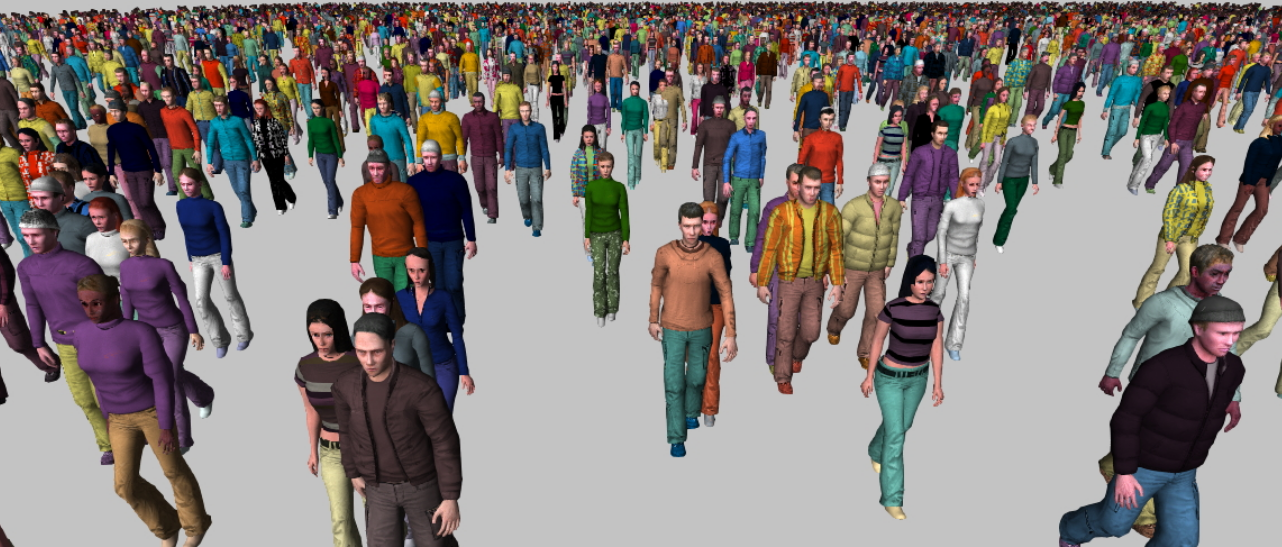
\includegraphics[scale=0.3]{images/crowd2}
		\caption{Animated crowd example, ~\cite{ruiz2013}.}
\end{figure}

\setcounter{page}{1} %Set page number
\columnsep 25.0pt %Column separation
\begin{multicols}{2} %Set for two columns

\section{Introduction}
\label{intro}

%Include why crowd simulation is interesting in films and videogames????
Crowds are encountered frequently, be it a large number of people in big shopping area, on a popular sports event, or at a demonstration.
Also non human crowds are quite common as well, such as schools of fish or flocks of birds.
There is a wide range of motives for their simulation.
Such as, in the \textit{film industry} where it is not always possible or economically viable to have a real crowd, in \textit{video games} as a crowd might be required in its virtual world and lastly, in \textit{disaster prevention and management} where they are used to aid in the decision making process as crowds provide new sources of data.\\

A crowd is much more than the collections of individuals that form it.
And as such the behaviour of the individuals could be affected by other members of the crowd.
History shows how in some cases crowd of people behave in a well organized manner, while in others its individual act selfishly abandoning all social norms.
When simulating this interactions with a naive approach, as the numbers of individuals in the crowd increase the computational cost of the interrelations calculation increments exponentially.\\

This problem has actually a number of clearly differentiated areas.
Firstly there is a \textit{crowd generation} problem, a modeller needs user-friendly tools in order to set up a scene in which a crowd is present.
Secondly the crowd is an evolving entity, so a \textit{crowd dynamics model} is required to govern the state of the crowd over time.
Thirdly, the model should be presented to the user, so a \textit{rendering} stage is needed.\\

Crowd simulation and rendering has been an active research area as early as 1987 with a simulation of flocks of birds by \cite{Reynolds1987}.
The author proved that a coherent global behaviour could be achieved by implementing a number of local rules in each entity.

\section{Classifications}

A clear line can be drawn between real-time simulation (games) and non real-time simulation (films).
Since the requirements for each simulation are quite different and so are the techniques used in each area.
However, with such a broad area, a more detailed exploration is required.
Consequently, each of the stages defined in section~\ref{intro} will be treated independently.

\subsection{Modelling Classifications}
\label{subsec:ModelClassification}

In order to simulate crowd behaviour a number of approaches have been proposed.
As they share certain similarities, they can be divided using a common criteria such as the simulation time  and the size of the modelled crowd.\\

Regarding time, we have short-term simulations, medium-term simulations and long-term simulations.
While in terms of size, a distinction can be made among small, medium and big size crowds.\\

The type of model used for the agents in the crowd can also be used as a criteria.
Therefore there are \textbf{entity based} simulations, where all individuals are homogeneous, or \textbf{agent based} simulations, where each individual is intelligent and autonomous.
Generally, agent based or entity based systems are used for small and medium crowds.\\

While for big size crowds, due to their challenging nature, \textbf{flow based} simulations are adopted as the most common approach.
In flow based simulations the discrete individual is disregarded in favour of a fluid based approach.
Evidently, this assumption looses effectiveness as the density of entities in the crowd decreases.
Hence, it will typically be considered only after a certain density threshold is met.\\

Lastly, \textbf{hybrid methods} are based on two or more of the afore mentioned techniques.
Their advantage lies in choosing the best model according to the situation or even directly mixing characteristics as needed. 

\subsection{Rendering Classifications}
\label{subsec:RenderingClassification}

Rendering techniques can be classified considering how they perform model reductions, since they have to be able to efficiently render the huge amounts of data needed for crowd simulation.\\

\textbf{Dynamic mesh decimation}, involves adopting simpler mesh representations.
\textbf{Dynamically generated impostors}, this procedure entails displaying 2D billboards with fixed poses instead of the full model.
\textbf{Point-rendering} techniques build multi-resolution representations using point samples from the mesh.
Since creating a unique individual for each entity in the crowd would be impractical, a common procedure in rendering crowds is to share the same render model among several entities.
Because this ``cloned'' models are visually undesirable, a method to infuse divergence in order to \textbf{achieve variety} is required. 

\section{Generating Crowds}

Before the crowd can be simulated or rendered it has to be generated.
Unfortunately, this task has not been researched as deeply as the rest.
In this stage the initial parameters at which the crowd operates are defined.
For example, crowd size, goals, ..., and can also include visual parameters such as color or models for the agents.\\

\cite{Ulicny2004} proposed a brush metaphor to manipulate crowds.
The author technique provides tools for the user in the form of a brush operator(create individuals, change color, etc) and then those tools can be used in the crowd world space.
Edited individuals in the crowd will be those in sight in the screen domain.
Therefore an intuitive approach is provided, as it is similar to what users are used to.
However it has certain limitations, such as lack of direct control over crowd behaviour or difficulty to select individuals in cluttered environments.\\

Some of the shortcomings of the previous work were met by \cite{Jordao2014}, whose method utilizes crowd patches.
Such patch areas define the crowd behaviour and can be edited through a sculpting metaphor, while also addressing the problem of populating vast empty areas efficiently.
What is more, crowd motion can be modified on the fly as the patches are editable in real time.
Nonetheless, individual paths cannot be controlled and only linear patch transformation was explored.

\section{Simulating Crowds}

As stated in section~\ref{intro}, following a naive approach leads to intractable computing times in simulations that handle more than a small sized crowd.
Below we describe in detail the approaches mentioned in section~\ref{subsec:ModelClassification}. 

\subsection{Entity Based}

\cite{Helbing2000} presented a model where individuals are represented as particles with velocity, mass and forces.
All individual goals are encoded as values in such components.
The model was designed to replicate pedestrian behaviour in panic situations.
Shortcomings are associated with the restricted goal of the simulation, such as difficult per group control and simplistic behaviour.\\

\cite{batty2003} introduced a similar pedestrian model although aimed at simulating carnivals and parades.
The author's model is based on a cellular automata, where an agent step is encoding as moving from the current cell to a neighbour cell.
This technique is constrained to evaluating safety policies and it only has an offline work mode.

\subsection{Agent Based}

\cite{helbing2002} did a complete study of a broad range scenarios in crowd behaviour, with special attention at panic versus not panic crowd behaviour.
A common pedestrian model applicable to all the situations was derived.\\

\cite{raupp2001} presented a three fold approach to agent based simulations: scripted behaviours, behavioural rules, with events and reactions, and external controls to guide the behaviour.
Controlling the complexity of the behaviours by group settings provides a flexible framework for crowd editing.
But complex individual behaviour was not been achieved.\\

More recent techniques add a counterflow paradigm, where agents not only take into account trail formation but also collision avoidance, \cite{heliovaara2012}.
Previous methods create unrealistic jams and collision in counterflow situations.
However this technique is able to solve them successfully.
Nevertheless, this model is still fails to account for other behaviours as it only concerned with counter-flow situations.

\subsection{Flow Based}

\cite{hughes2003} proposed a flow model method to simulate large crowds behaviour based on intelligent fluid flow.
An intelligent fluid tends to prefer certain paths, i.e. avoiding excessive congestive areas, achieving a more complete model for pedestrian simulation.
However, it would not take into account crowd flow in the individual speeds, therefore preventing lane formation.\\

The previous model was improved by \cite{treuille2006} with the addition of continuum dynamics.
Fixing the afore mention problems as well as undesirable oscillations in Hughes's model.
Like other flow based models, this technique fails to take into account individual variability.
Moreover it is limited to have a single common goal for all the characters.

\subsection{Hybrid Models}

\cite{Narain2009} presented a agent-fluid hybrid model.
Each agent has a preferred velocity and path, however on densely populated regions an incomprehensibility flow factor comes into play.
This factor acts by preventing agents from packing together too closely.\\

More recently \cite{lin2014} proposed also an agent-fluid hybrid solution to long-range collision avoidance.
When the density is below a certain threshold a discrete collision avoidance is used,
while after the threshold a fluid based lookahead algorithm controls the behaviour.
This technique shows advanced complex behaviour, such as a bigger group splitting in two to make space for a smaller group to go through it.
However it some cases it leads to unnatural groups separations.

\section{Rendering Crowds}

The main obstacle to overcome with crowd rendering is how to simplify the scene in order to be rendered in real or feasible time.
Hence, the goal in the following techniques is to reduce the computations in the rendering stage.
A common approach consist of applying a model complexity reduction that is still visually unnoticeable.
Bellow, we present in more detail the techniques commented in section~\ref{subsec:RenderingClassification}.

\subsection{Dynamic Mesh Decimation}

Progressive meshes were introduced by~\cite{Hoppe1996} as a compressed alternative to traditional meshes.
However, progressive meshes can be used as a coarser visual representation of the original mesh.
Provided that the decimation calculation is smaller than the total gain, there will be an increase in rendering performance.
Yet, the coarseness is limited if rendering quality is to be preserved.\\

Building on Hoppe's work, \cite{Hu2009} proposed a GPU implementation for progressive mesh refinement.
Anyhow, the author's implementation is more a prove of feasibility than a real improvement in performance.

\subsection{Dynamically Generated Impostors}
\label{subsec:DimGenImpostors}

Impostors are 2D pre-computed billboards used in place of the full 3D mesh model, thus reducing the cost of the rendering stage, as shown by~\cite{Aubel2000}.
However, when an impostor is rendered to an area larger than the impostor resolution, pixels from the impostor texture become noticeable.\\

%TODO Add drawback
~\cite{Millan2006} presented a GPU impostor implementation, which also used pseudo-instancing for further performance gains~\cite{zelsnack2004glsl}.
Yet, their implementation is only designed for a single GPU.\\

More recent advances were made by~\cite{Ghiletiuc2013} with a client-server impostor implementation in mobile devices.
Nevertheless, the bulk of the computation was still performed on the server side.

\subsection{Point-Rendering}

Point rendering uses a point cloud subset from the mesh model to reduce the complexity of the individuals in the crowd.
Using less points as the camera moves further away from the model.
\cite{Wand2002} showed that by using multi-resolution point sample rendering in key frame animations, the rendering time becomes independent from the complexity of the geometric model.\\

~\cite{Larkin2010} presented a point-rendering method that achieved real-time rendering by limiting the resources of the whole crowd, and sharing them with a level of detail value determined by a Delaunay triangulation. 
Each vertex in the triangulation has a density value that is used to calculate the number of points to render.
With small and medium crowds this technique works reasonably well.
However, with very large crowds the resources allocated for each instance can be insufficient.

\subsection{Achieving Variety}

There have been research into applying color variety, height change, accessories, animation variety to copies of individuals.
Since it is an inexpensive method to have a varied crowd.
Moreover, they rely on instancing, which is a desirable property,~\cite{zelsnack2004glsl}.\\

Crowds in specific situations has been simulated, for example \cite{deHeras2005} worked with a virtual Roman crowd in an urban environment.
In this paper they avoided computing each character’s mesh deformation using a precomputed deformed one for each frame. As well as applying color modulation accelerated hardware on instances of the same individual model.\\

\cite{ruiz2013} proposed a memory efficient method to generate new characters by varying skin color, clothes and body size.
The author's method involves a preprocessing stage and a run time stage.
In the first stage, assets are generated from the individuals, including texture maps, new animations, etc.
This stage is done per body part mesh to increase asset reusability.
While on the second stage new characters are animated using the previously generated assets.
However, the method is still not fully automatic and it needs pregenerated rigs.

% Topics to look for in papers are to be added in this area 
%- Color modulation
%- Texture variation
%- Shape deformation
%- Outfit creation
%- Animation diversity

\section{Conclusion}
We have seen an overview of the research techniques in crowd generation, simulation and rendering.
The generation and editing areas are still not sufficiently research as to provided easy to use tools.
However, important advances has been made, i.e. crowd brush metaphor presented by~\cite{Ulicny2004}.
On the simulation side there is a clear trend to abandon entity based simulations for agent based ones, as well as a hybrid method approaches.
Flow based simulations sacrifices too much detail, nevertheless hybrid approach seems to be addressing this issue.
But this methods are still not general enough and produce artificial outcomes in certain situations.
While on the rendering area, LOD techniques have been refined into research areas on their own.
Such as progressive meshes or point cloud rendering.
The use of instances with automatic colour, height or accessories variation optimizes the rendering stage.
Moreover, most of them produce reasonable results automatically.
In all the areas a lot of previous processing done by the CPU have been moved to the GPU.
This has approach has produced significant performance increases.
Still, a behavioural complex real-time simulation with easy editing and high quality rendering is still unachievable with the current techniques.

\bibliographystyle{apalike} %Close to Harvard style
\bibliography{template} %Include template.bib bibliography file
\end{multicols}
\end{document}
